\section{Design}
\label{sec:method}

\subsection{Overview}

We propose \textbf{Perceptually-Aware $\sigma$-zero}, which extends the original $\sigma$-zero objective with three complementary visual perception constraints. The overall loss function is:
\begin{align}
    \cL_{\text{total}} &= \cL_{\text{adv}} + \lambda_0 \cL_{\ell_0} + \lambda_{\infty} \cL_{\ell_\infty} \nonumber \\
    &\quad + \lambda_{\text{SSIM}} \cL_{\text{SSIM}} + \lambda_{\text{TV}} \cL_{\text{TV}},
    \label{eq:total_loss}
\end{align}
where each term is defined below.

\subsection{Loss Components}

\paragraph{Adversarial Loss.} We use the difference of logits (DL) loss:
\begin{equation}
    \cL_{\text{adv}} = \max(0, f_y(\x') - \max_{j \neq y} f_j(\x')),
\end{equation}
where $f_y$ is the logit for the true class $y$, and $\x' = \x + \deltaVec$.

\paragraph{$\ell_0$ Approximation.} Following~\cite{cina2025sigma}:
\begin{equation}
    \cL_{\ell_0} = \frac{1}{d} \sum_{i=1}^{d} \frac{\delta_i^2}{\delta_i^2 + \sigma}.
\end{equation}

\paragraph{$\ell_\infty$ Penalty.} To bound per-pixel perturbation magnitude:
\begin{equation}
    \cL_{\ell_\infty} = \max_i \abs{\delta_i}.
\end{equation}
This prevents any single pixel from undergoing extreme changes.

\paragraph{SSIM Loss.} To preserve structural similarity~\cite{wang2004image}:
\begin{equation}
    \cL_{\text{SSIM}} = 1 - \text{SSIM}(\x + \deltaVec, \x),
\end{equation}
where SSIM is computed using a Gaussian window of size $11 \times 11$ with $\sigma = 1.5$. The SSIM index measures luminance, contrast, and structural similarity between the original and perturbed images.

\paragraph{Multi-scale SSIM.} We extend SSIM to multiple scales for more comprehensive structural preservation:
\begin{equation}
    \cL_{\text{MS-SSIM}} = 1 - \sum_{s \in \mathcal{S}} w_s \cdot \text{SSIM}(\x^{(s)} + \deltaVec^{(s)}, \x^{(s)}),
\end{equation}
where $\mathcal{S} = \{1.0, 0.5, 0.25\}$ are down-sampling scales with weights $w = \{0.5, 0.3, 0.2\}$. Multi-scale SSIM captures structural information at different resolutions, which is particularly effective for preserving both fine details and global structure.

\paragraph{Total Variation Regularization.} To encourage spatial smoothness of the perturbation:
\begin{equation}
    \cL_{\text{TV}} = \frac{1}{d} \sum_{i,j} \left( \abs{\delta_{i+1,j} - \delta_{i,j}} + \abs{\delta_{i,j+1} - \delta_{i,j}} \right).
\end{equation}
TV regularization penalizes rapid spatial variations in the perturbation, discouraging scattered salt-and-pepper artifacts.

\subsection{Adaptive Weighting Scheme}

Fixed weights $\lambda_{\infty}, \lambda_{\text{SSIM}}, \lambda_{\text{TV}}$ may not be optimal throughout the optimization trajectory. Early stages benefit from aggressive attack (low constraints), while later stages should focus on refining visual quality (high constraints). We propose an adaptive weighting scheme:
\begin{equation}
    \lambda^{(t)} = \lambda_{\text{init}} \cdot \alpha(t),
\end{equation}
where $\alpha(t)$ is a scheduling function of the optimization progress. We consider three schedules:

\begin{itemize}
    \item \textbf{Linear:} $\alpha(t) = t / T$
    \item \textbf{Cosine:} $\alpha(t) = (1 - \cos(\pi t / T)) / 2$
    \item \textbf{Exponential:} $\alpha(t) = 1 - \exp(-3t / T)$
\end{itemize}

where $t$ is the current iteration and $T$ is the total number of iterations. The cosine schedule provides a smooth transition that we found most effective in practice.

\begin{figure*}[t]
    \centering
    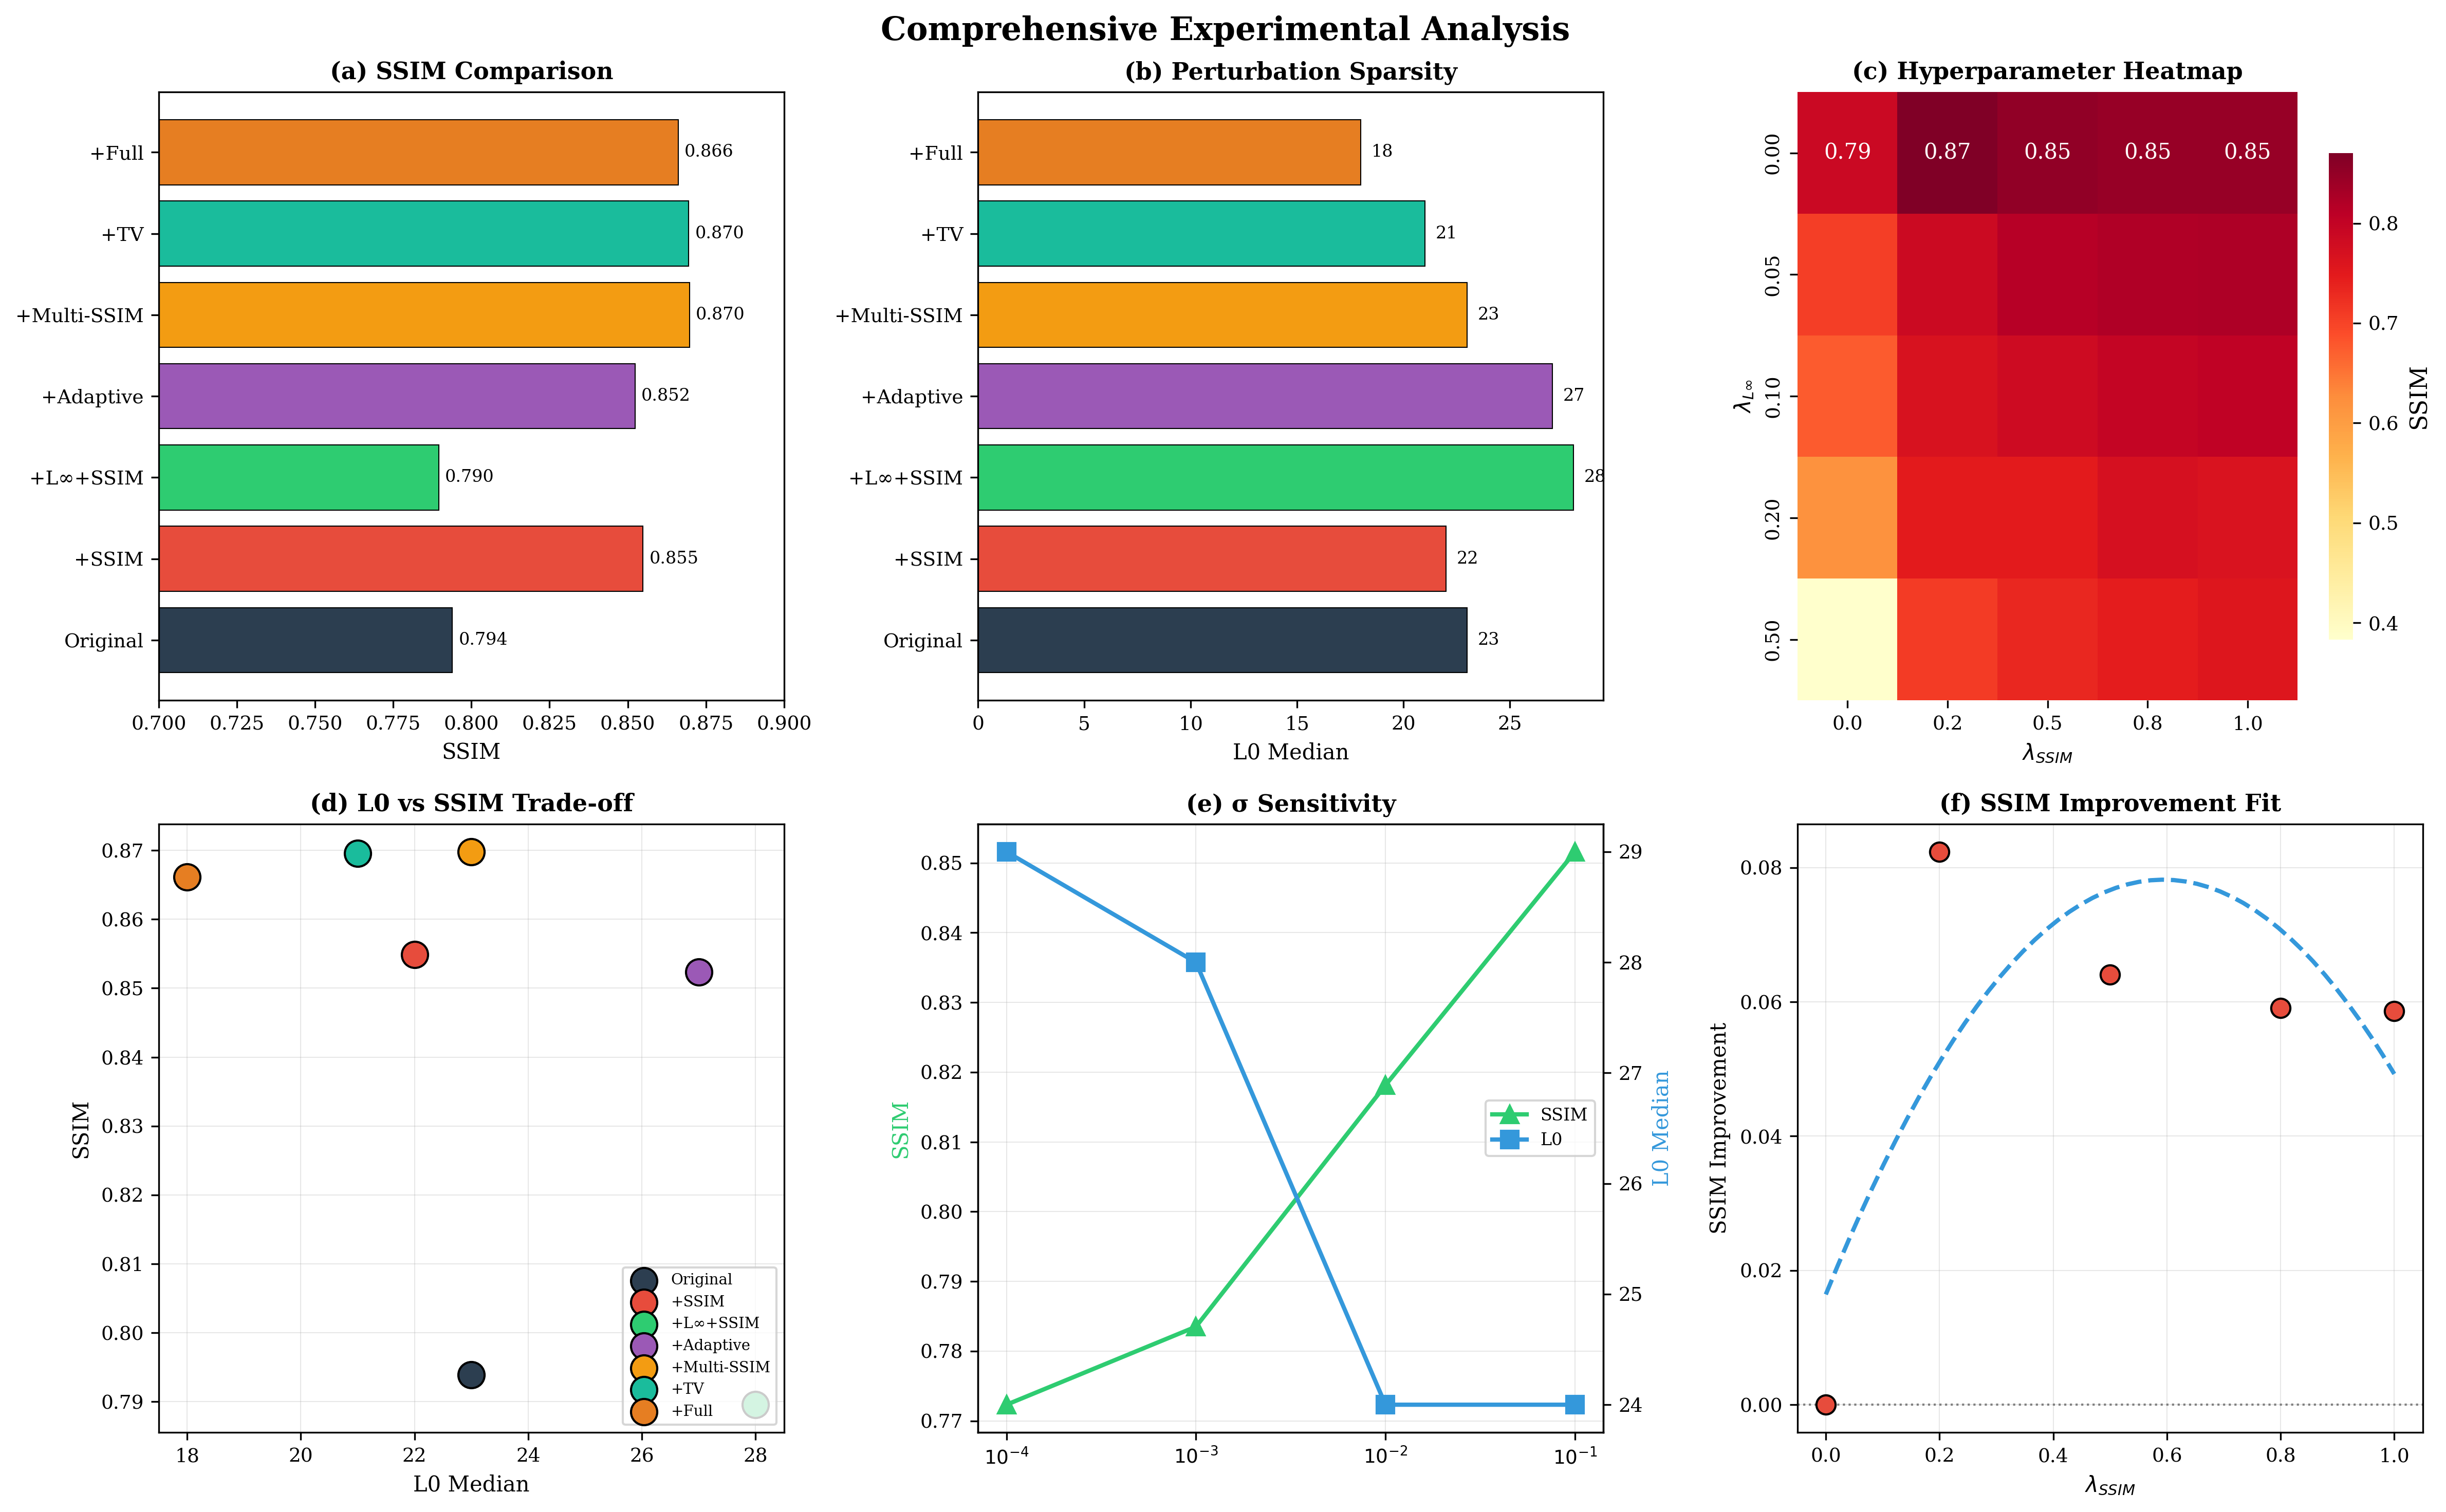
\includegraphics[width=0.95\textwidth]{figures/comprehensive_panel.png}
    \caption{Comprehensive experimental analysis: (a) SSIM comparison across methods, (b) perturbation sparsity (L0), (c) hyperparameter heatmap ($\lambda_{L\infty} \times \lambda_{\text{SSIM}}$), (d) L0 vs SSIM trade-off scatter plot, (e) $\sigma$ sensitivity analysis, (f) SSIM improvement fitting curve.}
    \label{fig:comprehensive}
\end{figure*}

\begin{table*}[t]
    \centering
    \caption{MNIST Results: Comparison of $\sigma$-zero variants on the MNIST dataset with SmallCNN (DDN robust training). All methods use 100 optimization steps and 50 test samples.}
    \label{tab:mnist_results}
    \begin{tabular}{lcccccc}
        \toprule
        \textbf{Method} & \textbf{ASR (\%)} $\uparrow$ & \textbf{L0 Median} $\downarrow$ & \textbf{L$\infty$ Mean} $\downarrow$ & \textbf{SSIM} $\uparrow$ & \textbf{SSIM $\Delta$} $\uparrow$ \\
        \midrule
        $\sigma$-zero (original) & 100.0 & 23.0 & 1.0000 & 0.7939 & --- \\
        \midrule
        + SSIM & 100.0 & 22.0 & 0.9997 & 0.8549 & +7.7\% \\
        + L$\infty$ + SSIM & 100.0 & 28.0 & 0.9947 & 0.7896 & -0.5\% \\
        + Adaptive & 100.0 & 27.0 & 0.9850 & 0.8523 & +7.4\% \\
        + Multi-scale SSIM & 100.0 & 23.0 & 0.9994 & \textbf{0.8698} & \textbf{+9.6\%} \\
        + TV & 100.0 & 21.0 & 0.9904 & 0.8695 & +9.5\% \\
        + Full (all) & 100.0 & \textbf{18.0} & 0.9952 & 0.8662 & +9.1\% \\
        \bottomrule
    \end{tabular}
\end{table*}

\subsection{Algorithm}

The complete algorithm is summarized in Algorithm~\ref{alg:perceptual_sigmazero}. The key modifications from the original $\sigma$-zero are highlighted with \textbf{[NEW]} markers.

\begin{algorithm}[t]
    \caption{Perceptually-Aware $\sigma$-zero}
    \label{alg:perceptual_sigmazero}
    \begin{algorithmic}[1]
        \REQUIRE Model $f$, input $\x$, label $y$, steps $T$, hyperparameters $\lambda_0, \lambda_\infty, \lambda_{\text{SSIM}}, \lambda_{\text{TV}}$
        \ENSURE Adversarial example $\x^*$
        \STATE Initialize $\deltaVec \leftarrow \mathbf{0}$, threshold $\tau \leftarrow \tau_0$
        \STATE Initialize optimizer (Adam) and scheduler (CosineAnnealing)
        \FOR{$t = 0$ to $T-1$}
            \STATE Compute adaptive weights: $\lambda^{(t)} = \lambda \cdot \alpha(t)$
            \STATE $\x' \leftarrow \x + \deltaVec$
            \STATE Compute logits: $\z \leftarrow f(\x')$
            \STATE Compute adversarial loss: $\cL_{\text{adv}} \leftarrow \text{DL}(\z, y)$
            \STATE Compute $\ell_0$ approximation: $\cL_{\ell_0} \leftarrow \sum \frac{\delta_i^2}{\delta_i^2 + \sigma}$
            \STATE \textbf{[NEW]} Compute $\ell_\infty$ penalty: $\cL_{\ell_\infty} \leftarrow \max_i \abs{\delta_i}$
            \STATE \textbf{[NEW]} Compute SSIM loss: $\cL_{\text{SSIM}} \leftarrow 1 - \text{SSIM}(\x', \x)$
            \STATE \textbf{[NEW]} Compute TV loss: $\cL_{\text{TV}} \leftarrow \text{TV}(\deltaVec)$
            \STATE Combine losses (Eq.~\ref{eq:total_loss})
            \STATE Backward pass and update $\deltaVec$
            \STATE Update dynamic threshold $\tau$
            \STATE Zero out components: $\delta_i \leftarrow 0$ if $\abs{\delta_i} < \tau$
            \STATE Clip: $\x + \deltaVec \in [0, 1]$
        \ENDFOR
        \RETURN $\x^* \leftarrow \x + \deltaVec_{\text{best}}$
    \end{algorithmic}
\end{algorithm}
